\documentclass[conference]{IEEEtran}
\IEEEoverridecommandlockouts
% The preceding line is only needed to identify funding in the first footnote. If that is unneeded, please comment it out.
\usepackage{cite}
\usepackage{amsmath,amssymb,amsfonts}
\usepackage{algorithmic}
\usepackage{graphicx}
\usepackage{textcomp}
\usepackage{xcolor}
\usepackage{hyperref}
%\usepackage{algorithm}
\usepackage{algorithm2e}
\usepackage{algorithmic}
\DeclareMathOperator*{\argmin}{arg\,min}
\def\BibTeX{{\rm B\kern-.05em{\sc i\kern-.025em b}\kern-.08em
    T\kern-.1667em\lower.7ex\hbox{E}\kern-.125emX}}
\begin{document}

\title{Efficient Hessian-Free Optimization of Deep Neural Networks
%\\
%{\footnotesize \textsuperscript{*}Note: Sub-titles are not captured in Xplore and
%should not be used}
%\thanks{Identify applicable funding agency here. If none, delete this.}
}

\author{\IEEEauthorblockN{Niklas Brunn}
\IEEEauthorblockA{\textit{Albert Ludwigs University of Freiburg} \\
\textit{Mathematical Institute}\\
Freiburg, Germany \\
niklasbrunn@web.de}
\and
\IEEEauthorblockN{No\"{e}l E. Kury}
\IEEEauthorblockA{\textit{Albert Ludwigs University of Freiburg} \\
\textit{Mathematical Institute}\\
Freiburg, Germany \\
nekury@wkury.de}
\and
\IEEEauthorblockN{Clemens A. Schächter}
\IEEEauthorblockA{\textit{Albert Ludwigs University of Freiburg} \\
\textit{Mathematical Institute}\\
Freiburg, Germany \\
clemens.schaechter@live.com}
}

\maketitle
\thispagestyle{plain}
\pagestyle{plain}

\begin{abstract}
This report is a written elaboration of a project which was developed in the lecture Numerical Optimization in the winter term 21/22 at the Albert-Ludwigs-University of Freiburg.\\
We discuss a $2^{\text{nd}}$-order optimization method for training deep neural networks using the Generalised Gauss Newton Matrix as an approximation for the Hessian of the objective loss function. This optimization method is superior to $1^{\text{st}}$-order methods, which uses only the gradient of the objective loss function with respect to the Deep Neural Networks`s parameters, in the sense that fewer iterations are required until convergence. In addition, we present an implementation of the method using Python 3, Tensorflow and examine results using a simulated simple dataset and the MNIST dataset.
\end{abstract}

\section{Introduction} 
Deep Neural Networks (DNNs) are one of the main components of Deep Learning which is a subfield of Machine Learning. When training a DNN, the network parameters are updated according to certain rules, which we call the DNN optimization method. By default, the Stochastic Gradient Descent (SGD) method is used as the optimization method. This is a $1^{\text{st}}$-order optimization method in which only the negative gradient of the object loss function (OL) with respect to the network parameters is used to update the current parameters.
One problem of SGD is that pathological curvature of the OL is not considered. This means that the method can get stuck in saddle points, or often converges very slowly in environments with pathological curvature. 
$2^{\text{nd}}$-order optimization methods take into account the curvature of the OL and can thus circumvent such problems, but they are costly in time because second order derivatives must be computed for this purpose. 
We want to use a version of Newton's method for DNN optimization as presented in [4].
The method presented there uses an approximation of the Hessian matrix, which is positive definite, and thus allows the use of the Conjugate Gradient (CG) method for determining parameter updates. We will therefore go into more detail on the individual problems of standard Newton updates and the improvements proposed for them in order to ensure efficiency.
We also explain how to implement the method in Python 3 with Tensorflow, using the Automatic Differentiation commands provided in the package for forward automatic differentiation (FAD) and backward automatic differentiation (BAD), and provide the reader our own implementation of the method \href{https://github.com/NiklasBrunn/Hessian_Free_Optimization_of_Deep_Neural_Networks}{(link to our Github Repository)}. We will show, using the experiments presented here and our own implementation, that the method does indeed converge in fewer epochs, but is still significantly slower in time than SGD.


\section{Optimization of Deep Neural Networks}
In this section, we introduce the necessary mathematical notations for optimizing DNNs, formulate the Parameter optimization task as a Nonlinear Programmming problem (NLP) and explain tricks for the OL, which will be useful later when implementing the presented method.\\

\subsection{Deep Neural Networks}
As one of the main components of Deep Learning, DNNs are function approximators that can approximate any continuous function arbitrarily well. Given a dataset of observation pairs $D =\{(x_{i}, y_{i})_{1\leq i\leq N}\}$ with input ${x}$ and corresponding target $y$, the optimization task is to find optimal parameters such that given an observation $x$, the DNN`s evaluation with current parameters is approximatively the coressponding observed target $y$.  Whenever we use the designation
DNN we actually mean the realisation of a DNN given an input $x$, which is a mapping
\begin{align}
\mathrm{R}_{x}(\theta):\mathbb{R}^{d}\rightarrow\mathbb{R}^{m},
\end{align}
where $\theta$ is a vector containing the parameters of the DNN and $\Theta^{d}=\mathbb{R}^{d}$ denotes the parameter space with usually $d >> m$. We shortly write 
\begin{align} 
\hat{y}_{x} := \mathrm{R}_{x}(\theta)
\end{align}
for the Output of a DNN given an input $x$ with current parameters $\theta$. In detail $\mathrm{R}_{x}$ is an alternating concatenation of a fixed number of affine and nonlinear mappings, where the parameter vector $\theta$ is the collection of every entry of all matrices and vectors in the affine mappings. The affine mappings are called Layers and the nonlinear mappings are called activation functions in the Machine Learning literature and are always applied element-wise to the output of the preceding Layers. %\\
%(For a more detailed introduction to DNNs, we provide additional material in the Appendix)\\
Within this report, we also asume that there is no further activation function for DNNs after the last layer but allow that outside the DNN a further activation function $\text{akt}:\mathbb{R}\rightarrow\mathbb{R}$ can be placed after the output of the DNN. This allows us to use technical tricks that later favor the implementation.
In that case we denote the Output of the afterwards element-wise application of an activationfunction to the output of a DNN with
\begin{align}
z_{x} := \text{akt}(\hat{y}_{x}) = \text{akt}(\mathrm{R}_{x}(\theta)).
\end{align}

\subsection{Loss functions}
For the optimization we need a good optimization criterion in the form of a scalar-valued loss function
\begin{align}
&\mathrm{L}:\mathbb{R}^{m}\rightarrow \mathbb{R}^{+};\\
&(\hat{y}_{x}, y)\mapsto \mathrm{L}_{y}(z_{x}) := \mathrm{L}(z_{x}, y),
\end{align}
which is asumed to be at least twice continuous-differentiable. The loss can be seen as a feedback signal, how well the DNN fits the observation data with its current parameters. Choosing a good loss function is one of the most important tasks in the optimization of DNNs. For example, in multi-classification tasks, the loss function used is the corssentropy loss function with previous softmax-activation function and for regression we typically use the squared error loss function with previous identity-activation function.

\subsection{Network training formulated as a NLP}
Parameter optimization of a DNN can be formulated as an unconstrained NLP. Therefore we define the OL as a mapping which calculates the empirical loss of the DNN`s output with current parameters $\theta$ given the input $x$ and the corresponding target $y$
\begin{align}
&f_{D}:\Theta^{d}\rightarrow\mathbb{R}^{+};\\
\theta\mapsto f_{D}(\theta) &:= \mathbb{E}_{D}[\mathrm{L}_{y}(z_{x})] =  \frac{1}{N}\sum_{j = 1}^{N}\mathrm{L}_{y_{j}}(z_{x_{j}}).
\end{align}
Thus we get the unconstrained NLP formulation
\begin{align}
\argmin_{\theta\in\Theta^{d}}\quad f_{D}(\theta),
\end{align}
where $\theta$ denotes the decision variable and $f_{D}$ the objective function of the NLP.
Further, if we consider only one observation $(x, y)$ from the observation data set $D$, then we briefly write  $f_{x, y}$ for the corresponding OL. Note that for DNNs the above formulated NLP is typically nonconvex due to the nonconvexity of the OL.

\subsection{Matching loss functions}
For later purposes we need to calculate the Jacobian or. the gradient of the OL with respect to the DNN`s parameters. For simplicity we consider the OL for only one pair of observations
\begin{align}
\frac{\partial}{\partial\theta}f_{x, y}(\theta) = \mathrm{J}_{f_{x, y}}.
\end{align}
Note that due to the linearity of the derivative, the results can be extended without problems to the case where the whole data set or a batched version of the whole data set is considered.
Applying the chain rule we can rewrite the Jacobian in (9) to
\begin{align}
\mathrm{J}_{f_{x, y}} &= \mathrm{J}_{\mathrm{L}_{y}\circ \:\text{akt} \:\circ\:\mathrm{R}_{x}} = \mathrm{J}_{\mathrm{L}_{y}} \: \mathrm{J}_{\text{akt}} \: \mathrm{J}_{\mathrm{R}_{x}},\\
\mathrm{J}_{f_{x, y}}^{\mathrm{T}} &= \mathrm{J}_{\mathrm{R}_{x}}^{\mathrm{T}} \: \mathrm{J}_{\text{akt}}^{\mathrm{T}} \: \mathrm{J}_{\mathrm{L}_{y}}^{\mathrm{T}}.
\end{align}
As introduced in [8], we also make use of the so-called matching loss functions, where we say that a loss function $\mathrm{L}$ matches the output-non-linearity $\text{akt}$ if
\begin{align}
\frac{\partial}{\partial\hat{y}_{x}}\left(\mathrm{L}_{y}\circ \text{akt}\right)^{\mathrm{T}}(\hat{y}_{x})= \mathrm{J}_{\mathrm{L}_{y}\circ \:\text{akt}}^{\mathrm{T}} = A\: z_{x} + b,
\end{align}
for a matrix $A$ and a vector $b$ which both do not depend on the parameters $\theta$.
The concept of matching loss functions will helpe us later in the implementation of the method. We will also see that many of the well known loss functions used for DNN optimization match their output-nonlinearity, e.g. the squared error loss function and crossentropy loss function with previous softmax-activation function.


\section{Hessian-Free optimization method}
In this section we want to give the reader a compact presentation of the different components used in the presented method. We will briefly review Newton`s method and go over the advantages and disadvantages of the usage of the Hessian matrix, and then introduce the necessary theory for the efficient $2^{\text{nd}}$-order optimization method. For a more detailed introduction in Newton-type optimization we refer the reader to [2] (Chapter 7), and [4] for details about the problems with pathological curvature. 

\subsection{Newton's method}\label{AA}
Newton`s method is an optimization method, where we update the decition variables of a NLP iteratively by
\begin{align}
 \theta_{k+1} = \theta_{k} -\mathrm{H}_{f_{x, y}}^{-1}\:\mathrm{J}_{f_{x, y}}^{\mathrm{T}},
\end{align}
where $\mathrm{H}_{f_{x, y}}$ denotes the always symmetric Hessian matrix of the OL with respect to the current DNN`s parameters $\theta$ in the $k+1$-th step. This approach is motivated by minimizing the local quadratic approximation
\begin{align}
q(\theta + \delta)_{x, y} &:= f_{x, y}(\theta) + \mathrm{J}_{f_{x, y}}^{\mathrm{T}}\:\delta + \frac{1}{2}\:\delta^{\mathrm{T}}\:\mathrm{H_{f_{x, y}}}\:\delta\\
&\approx f_{x, y}(\theta + \delta)
\end{align}
with respect to $\delta$. 
Respecting informations about the curvature of the OL, using the Hessian can in contrast to the usage of gradient descent lead to convergence in much lesser iterations because it rescales the gradient of the OL in every step by using information about the local curvature of the OL.

\subsection{Problems with the Hessian}
We implicitly asume in every step of the Newton`s methode that the Hessian matrix is invertible, which in our case is very rare in the task of optimizing DNN`s parameters and even if the Hessian is invertible, we cannot ensure converges to a local minimum, since the Hessian usually does not have to be positive semidefinite either. Apart from that, the Hessian matrix has $d^{2}$ entries consisting of second-order partial derivatives, which makes it incredibly expensive to calculate, asuming $d>>m$. For this reason, the direct application of Newton's method to our task is inappropriate and we must first make some modifications to ensure an efficient application of Newton`s method..

\subsection{The Generalized Gauss Newton Matrix}
As a first improvement, we no longer use the Hessian matrix itself, but the Generalized Gauss Newton matrix (GGN), which is an approximation of the Hessian matrix
\begin{align}
\mathrm{G}_{f_{x, y}} := \mathrm{J}_{\hat{y}_{x}}^{\mathrm{T}}\:\mathrm{H}_{\mathrm{L_{y}\circ\:\text{akt}}}\:\mathrm{J}_{\hat{y}_{x}},
\end{align}
with $\mathrm{H}_{\mathrm{L_{y}\circ\:\text{akt}}}$ denoting the Hessian of $\mathrm{L_{y}\circ\:\text{akt}}$ with respect to the DNN`s output $\hat{y}_{x}$ and $\mathrm{J}_{\hat{y}_{x}}$ denoting the Jacobian of the DNN`s output with respect to its parameters.
This representation is motivated by the fact that in the representation of the complete Hessian matrix
\begin{align}
\mathrm{H}_{f_{x, y}} = \mathrm{J}_{\hat{y}_{x}}^{\mathrm{T}}\:\mathrm{H}_{\mathrm{L_{y}\circ\:\text{akt}}}\:\mathrm{J}_{\hat{y}_{x}}\:\sum_{j = 1}^{m}\left(\left(\mathrm{J}_{\mathrm{L}_{y}\circ \:\text{akt}}^{\mathrm{T}}\right)_{j}\cdot\mathrm{H}_{(\hat{y}_{x})_{j}}\right),
\end{align}
where $\mathrm{H}_{(\hat{y}_{x})_{j}}$ denotes the Hessian of the DNN`s  $j$-th output, the last sum-term vanishes if 
\begin{align}
\left(\mathrm{J}_{\mathrm{L}_{y}\circ \:\text{akt}}^{\mathrm{T}}\right)_{j}\approx 0\:\lor\:\mathrm{H}_{(\hat{y}_{x})_{j}} \approx 0.
\end{align}
which in the first case of (18) means that the DNN represents the targets well.  Moreover, by construction, the GGN is a symmetric matrix and is positive semidefinite if $\mathrm{L_{y}\circ\:\text{akt}}$ is convex since for every $v\in\mathbb{R}^{d}$ it holds that
\begin{align}
v^{\mathrm{T}}\:\mathrm{G}_{f_{x, y}}\:v &= v^{\mathrm{T}}\:\left( \mathrm{J}_{\hat{y}_{x}}^{\mathrm{T}}\:\mathrm{H}_{\mathrm{L_{y}\circ\:\text{akt}}}\:\mathrm{J}_{\hat{y}_{x}}\right)\:v\\
&= \left(\mathrm{J}_{\hat{y}_{x}\:v}\right)^{\mathrm{T}}\:\mathrm{H}_{\mathrm{L_{y}\circ\:\text{akt}}}\left(\mathrm{J}_{\hat{y}_{x}\:v}\right) \\
&\geq 0.
\end{align}
For more information about the GGN we recommend chapter 8 in [5] .

\subsection{Levenberg-Marquardt algorithm }
Even if we would use the GGN insted of the Hessian in (13), which results in much faster runtime in contrast to the usage of the Hessian and is much more memory efficient, we cannot ensure invertibility. Thus it it sometimes not possible to find a solution of the linear system
\begin{align}
\mathrm{G}_{f_{x, y}}\cdot(\theta_{k+1} - \theta_{k}) = -\mathrm{J}_{f_{x, y}}^{\mathrm{T}},
\end{align}
which is equivalent to the system stated in (13) using the GGN insted of the Hessian.
For that reason we use a damped version of the GGN (DGGN) where we add an diagonal matrix with positive values on the diagonal, e.g.
\begin{align}
\mathrm{DG}_{f_{x, y}} := \mathrm{G}_{f_{x, y}} + \lambda\cdot\mathrm{I}^{d\times d},
\end{align}
with $\mathrm{I}^{d\times d}$ denoting the $d\times d$ unit matrix and some $\lambda>0$.
The DGGN constructed in this way is then actually invertible and positiv definite. 
To see this we consider the decomposition
\begin{align}
\mathrm{G}_{f_{x, y}} = \mathrm{U}\:\Lambda\:\mathrm{U}^{\mathrm{T}},
\end{align}
with an orthogonal Matrix $\mathrm{U}\in\mathbb{R}^{d\times d}$ and a diagonal Matrix $\Lambda\in\mathbb{R}^{d\times d}$ which on the diagonal entries contains the nonnegative eigenvalues of the GGN. This decomposition exists because the GGN is symmetric and positive semidefinite. Further it holds that
\begin{align}
\mathrm{DG}_{f_{x, y}} &= \mathrm{U}\:\Lambda\:\mathrm{U}^{\mathrm{T}} + \lambda\cdot\mathrm{I}^{d\times d}\\
&= \mathrm{U}\:\Lambda\:\mathrm{U}^{\mathrm{T}} + \mathrm{U}\:\lambda\cdot\mathrm{I}^{d\times d}\:\mathrm{U}^{\mathrm{T}}\\
&= \mathrm{U}\:\left(\Lambda + \lambda\cdot\mathrm{I}\right)\:\mathrm{U}^{\mathrm{T}}
\end{align}
where the Matrix $\left(\Lambda + \lambda\cdot\mathrm{I}\right)$ is a diagonal one with only positive entries on the diagonal. Therefore the determinant of the produkt of the matrices in the last term is positive and as a consequence we get that the DGGN is positive definite and invertible.
Note that a choice of $\lambda>>0$ leads to a Newton step where we would nearly not move away from our current parameters, while a choice of $\lambda\approx 0$ leads to a full step using the GGN (see also in [2], chapter 6.7). In practice, we update the value $\lambda$ after each iteration step according to certain conditions which we will explain in more detail later.

\subsection{Conjugate Gradient method}
\textbf{TODO ... (CG Erklären, R-Op. und effiziente Matrix-V-P., CG-Methode Extras erklären)}
For an efficient approximation of the parameter updates we do not compute the left term of the equation stated in (13) but instead use the CG method to iteratively approximate the solution of the linear system stated in (22), where we replace the GGN with the DGGN. Given a positive definite and symmetric matrix $A\in \mathbb{R}^{n\times n}$ we can approximate the unique solution of the linear system 
\begin{align}
A\:x = b
\end{align}
within 
\\\textbf{TODO ... (CG Erklären, R-Op. und effiziente Matrix-V-P., CG-Methode Extras erklären)}

\subsection{Mini-batches}
If we are facing a large observation data set with $N>>0$, it is common to split the data set into batches $\mathrm{M}\subset\mathrm{D}$ containing only a few random samples $M<<N$ of the entire data and apply the optimization method to each of the generated batches for each iteration. The partition of $\mathrm{D}$ into smaler batches is called a mini-batch szenario, where $M$ denotes the batchsize of the mini-batches. For each mini-batch $\mathrm{M}$ the DGGN in (23) becomes
\begin{align}
\mathrm{DG}_{f_{\mathrm{M}}} := \frac{1}{M}\sum_{(x, y)\in \mathrm{M}}^{}\mathrm{G}_{f_{x, y}} + \lambda\cdot\mathrm{I}^{d\times d}.
\end{align}
As mentioned in [3], the batch size should be relatively large to capture enough information about the curvature of the OL. 

\section {Implementation}
(TODO: matching loss für die Experimente, GGN Matrix für die Experimente, Lambda-Berechnungsregel, Minibatches, ...)
\subsection{Autodiff}
...
\subsection{Tensorflow}
...

\subsection{Figures and Tables}
\paragraph{Positioning Figures and Tables} Place figures and tables at the top and 
bottom of columns. Avoid placing them in the middle of columns. Large 
figures and tables may span across both columns. Figure captions should be 
below the figures; table heads should appear above the tables. Insert 
figures and tables after they are cited in the text. Use the abbreviation 
``Fig.~\ref{fig}'', even at the beginning of a sentence.

\begin{table}[htbp]
\caption{Table Type Styles}
\begin{center}
\begin{tabular}{|c|c|c|c|}
\hline
\textbf{Table}&\multicolumn{3}{|c|}{\textbf{Table Column Head}} \\
\cline{2-4} 
\textbf{Head} & \textbf{\textit{Table column subhead}}& \textbf{\textit{Subhead}}& \textbf{\textit{Subhead}} \\
\hline
copy& More table copy$^{\mathrm{a}}$& &  \\
\hline
\multicolumn{4}{l}{$^{\mathrm{a}}$Sample of a Table footnote.}
\end{tabular}
\label{tab1}
\end{center}
\end{table}

\begin{figure}[htbp]
\centerline{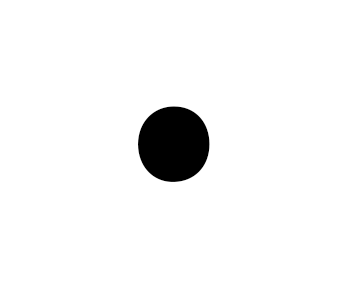
\includegraphics{fig1.png}}
\caption{Example of a figure caption.}
\label{fig}
\end{figure}

Figure Labels: Use 8 point Times New Roman for Figure labels. Use words 
rather than symbols or abbreviations when writing Figure axis labels to 
avoid confusing the reader. As an example, write the quantity 
``Magnetization'', or ``Magnetization, M'', not just ``M''. If including 
units in the label, present them within parentheses. Do not label axes only 
with units. In the example, write ``Magnetization (A/m)'' or ``Magnetization 
\{A[m(1)]\}'', not just ``A/m''. Do not label axes with a ratio of 
quantities and units. For example, write ``Temperature (K)'', not 
``Temperature/K''.

\section{Experiments}
TODO: ALGORITHMS (FAST-MAT-VEC-Pseudocode und CG-Pseudocode)

\RestyleAlgo{ruled}
\begin{algorithm}
	\SetKwInOut{Input}{Input}
	\SetKwInOut{Output}{Output}
	\SetKwInOut{CG}{\textbf{pre-CG-result}}
	\SetKwInOut{LAM}{\textbf{$\lambda$-update($\mathrm{M}$, $\Delta\theta_{k+1}$, $\lambda$)}}
	\caption{Hessian-Free pseudocode for (8)}\label{alg:one}
	\Input{$\mathrm{D}$, $\theta_{0}$, $\lambda$, epochs}
    \For{epoch in epochs}{
    	$k\gets 0$\\
	    \For{$(x, y)$ in $\mathrm{D}$}{
	        $\mathrm{J}_{f_{x, y}}^{\mathrm{T}}(\theta_{k})\:$(compute with BAD)\\
            \CG{$\Delta\theta_{k+1}$}
            $\theta_{k+1}\gets \theta_{k} + \Delta\theta_{k+1}$\\
            \LAM{$\lambda$}
            $k\gets k+1$
        }	
       $\theta_{0} \gets \theta_{N}$
    }
    \Output{$\theta^{trained}$}
\end{algorithm}

\begin{algorithm}
	\SetKwInOut{Input}{Input}
	\SetKwInOut{Output}{Output}
	\SetKwInOut{CG}{\textbf{pre-CG-result}}
	\SetKwInOut{LAM}{\textbf{$\lambda$-update($\mathrm{M}$, $\Delta\theta_{k+1}$, $\lambda$)}}
	\caption{(Mini-batch)-Hessian-Free pseudocode for (8)}\label{alg:two}
	\Input{$\mathrm{D}_{batched}$, $M$, $\theta_{0}$, $\lambda$, epochs}
	\For{$epoch$ in epochs}{
		$k\gets 0$\\
		\For{$\mathrm{M}$ in $\mathrm{D}_{batched}$}{
		    $\mathrm{J}_{f_{\mathrm{M}}}^{\mathrm{T}}(\theta_{k})\:$(compute with BAD)\\
			\CG{$\Delta\theta_{k+1}$}
			$\theta_{k+1}\gets \theta_{k} + \Delta\theta_{k+1}$\\
			\LAM{$\lambda$}    
			$k\gets k+1$
		}
	    $\theta_{0}\gets \theta_{M}$	
	}
    \Output{$\theta^{trained}$}
\end{algorithm}

\begin{algorithm}
	\SetKwInOut{Input}{Input}
	\SetKwInOut{Output}{Output}
	\SetKwInOut{CG}{\textbf{pre-CG-result}}
	\SetKwInOut{LAM}{\textbf{$\lambda$-update}}
	\SetKwInOut{FMV}{\textbf{fast-mat-vec-out($\mathrm{M}$, $\Delta\theta_{k+1}$, $\lambda$)}}
	\caption{Condition for $\lambda$-updates}\label{alg:three}
	\Input{$\mathrm{M}$, $\Delta\theta_{k+1}$, $\lambda$}
	\FMV{$\mathrm{DG}_{f_{\mathrm{M}}}\:\Delta\theta_{k+1}$}
	$A\gets\mathrm{DG}_{f_{\mathrm{M}}}\:\Delta\theta_{k+1}$\\
		\text{}\\
	$\rho\gets \frac{f_{\mathrm{M}}(\theta_{k}+\Delta\theta_{k+1})\:-\: f_{\mathrm{M}}(\theta_{k})}{\mathrm{J}_{f_{\mathrm{M}}}^{\mathrm{T}}\cdot\Delta\theta_{k+1} + \frac{1}{2}\Delta\theta_{k+1}^{\mathrm{T}}\cdot A}$\\
	\text{}\\
	\If{$\rho<\frac{1}{4}$}{$\lambda\gets \frac{3}{2}\:\lambda$}
	\ElseIf{$\rho>\frac{3}{4}$}{$\lambda\gets \frac{2}{3}\:\lambda$}
	\Output{$\lambda$}
\end{algorithm}

\begin{algorithm}
	\SetKwInOut{Input}{Input}
	\SetKwInOut{Output}{Output}
	\SetKwInOut{CG}{\textbf{pre-CG-result}}
	\SetKwInOut{LAM}{\textbf{$\lambda$-update($\mathrm{M}$, $\Delta\theta_{k+1}$, $\lambda$)}}
	\caption{Fast matrix-vector produkts (DGGN multiplied with an arbitrary vector $v$)}\label{alg:four}
	\Input{$\mathrm{M}$, $v$, $\lambda$}
	$\mathrm{G}_{f_{\mathrm{M}}}\:v$ (compute with FAD and BAD)\\
	$\mathrm{DG}_{f_{\mathrm{M}}}\: v \gets \mathrm{G}_{f_{\mathrm{M}}}\: v + \lambda\cdot\mathrm{I}^{d\times d}\:v$\\
	\Output{$\mathrm{DG}_{f_{\mathrm{M}}}\: v$}
\end{algorithm}

\begin{algorithm}
	\SetKwInOut{Input}{Input}
	\SetKwInOut{Output}{Output}
	\SetKwInOut{CG}{\textbf{pre-CG-result}}
	\SetKwInOut{LAM}{\textbf{$\lambda$-update($\mathrm{M}$, $\Delta\theta_{k+1}$, $\lambda$)}}
	\caption{(preconditioned) CG method}\label{alg:five}
	
\end{algorithm}

\subsection{Simple simulated data}
...

\subsection{MNIST}
...

\section{Conclusion}
...

\section*{Acknowledgment}
We want to thank the lecture assistant Florian Messerer for suggesting this topic for the project and giving us some sources to research. 


\begin{thebibliography}{00}
\bibitem{b1} M. Abadi, A. Agarwal, P. Barham, E. Brevdo,
Z. Chen, C. Citro, G. S. Corrado, A. Davis,
J. Dean, M. Devin, S. Ghemawat, I. Goodfellow,
A. Harp, G. Irving, M. Isard, R. Jozefowicz, Y. Jia,
L. Kaiser, M. Kudlur, J. Levenberg, D. Mané, M. Schuster,
R. Monga, S. Moore, D. Murray, C. Olah, J. Shlens,
B. Steiner, I. Sutskever, K. Talwar, P. Tucker,
V. Vanhoucke, V. Vasudevan, F. Viégas,
O. Vinyals, P. Warden, M. Wattenberg, M. Wicke,
Y. Yu, and X. Zheng.
TensorFlow: Large-scale machine learning on heterogeneous systems, Software available from tensorflow.org, 2015	
\bibitem{b2} M. Diehl, "Lecture Notes on Numerical Optimization (Preliminary Draft)", Albert Ludwigs University of Freiburg, September 29, 2017	
\bibitem{b3} M. Gargiani, A. Zanelli, M. Diehl, F. Hutter, "On the Promise of the Stochastic Generalized Gauss-Newton Method for Training DNNs",  arXiv:2006.02409v4, June 9, 2020 
\bibitem{b4} J. Martens, "Deep learning via Hessian-free optimization", University of Toronto, Ontario, M5S 1A1, Canada, 2010
\bibitem{b5} J. Martens, "New Insights and Perspectives on the Natural Gradient Method", Jurnal of Machine Learning Research 21, arXiv:1412.1193v11, September 19, 2020
\bibitem{b6} J. Martens, I. Sutskever, "Training Deep and Recurrent Networks with Hessian-Free Optimization", In: G. Montavon, G.B. Orr, KR. Müller (eds), Neural Networks: Tricks of the Trade. Lecture Notes in Computer Science, vol 7700. Springer, Berlin, Heidelberg, 2012
\bibitem{b7} B. A. Pearlmutta, "Fast Exact Multiplication by the Hessian", Neural Computation, June 9, 1993
\bibitem{b8} N. N. Schraudolph, "Fast Curvature Matrix-Vector Products for Second-Order
Gradient Descent", Neural Computation, August 2002
\bibitem{b9} G. Van Rossum, F. L. Drake, Python 3 Reference Manual. Scotts Valley, CA: CreateSpace, 2009
\end{thebibliography}

\end{document}
